\documentclass[ 11pt]{article}
\usepackage[utf8]{inputenc}
\usepackage[a4paper,width=160mm,top=25mm,bottom=25mm]{geometry}
\usepackage{graphicx} 

\title{European Commission}
\author{}
\date{June 2023}

\begin{document}

\maketitle

Problem with 'S.A.' node. 
\section{Model using hypergraphs or graphs?}

\subsection{Hpyergraph}
Number of hyperedges : 11214\\
Number of entities (nodes): 4541\\
Number of edges in a bipartite graph 32501 \\
Mean cardinality : 2.90\\
Std cardinality : 2.25\\
 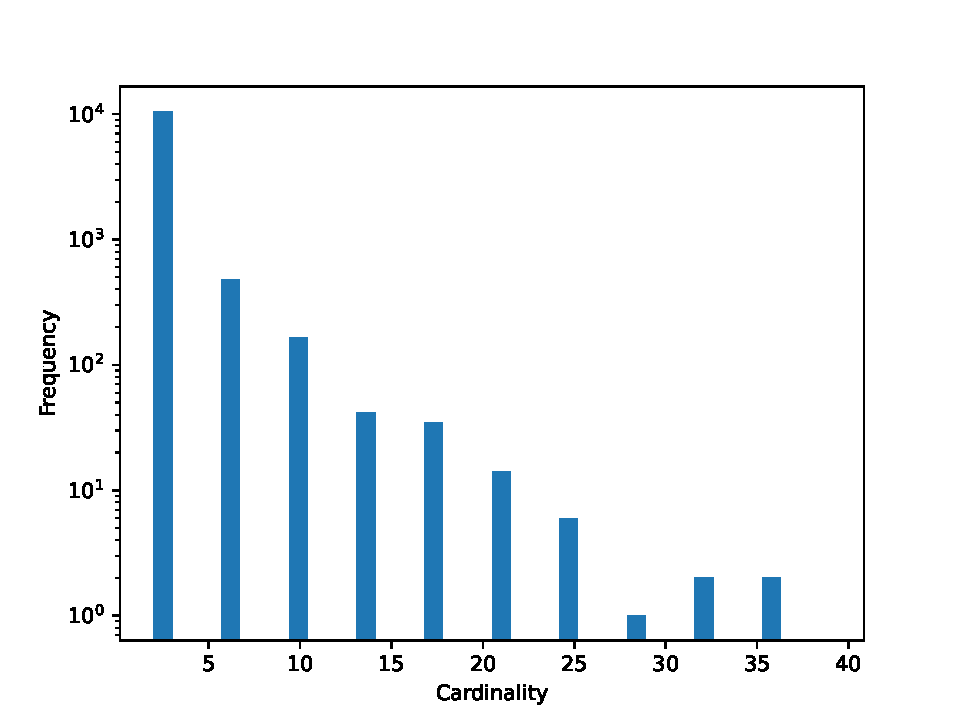
\includegraphics[scale=0.5]{../Programs/Figures/hist_Cardinality.pdf}

- Correlation between centralities of hyperedges.\\

\begin{tabular}{|c|ccc|}
\hline
			&Betweenness  &Cardinality  &Closeness \\
			\hline
Betweenness     &1.000000     &0.751155  & 0.528181 \\
Cardinality     &0.751155     &1.000000  & 0.417462 \\
Closeness       &0.528181    &0.417462  & 1.000000 \\
\hline
\end{tabular}  \\

     $\Rightarrow$  big hyperedges have a high cardinality
     
\subsection{Graph}
Number of entities (nodes): 4541\\
Number of edges : 35139 \\


\section{Centralities}
\subsection{Degree}
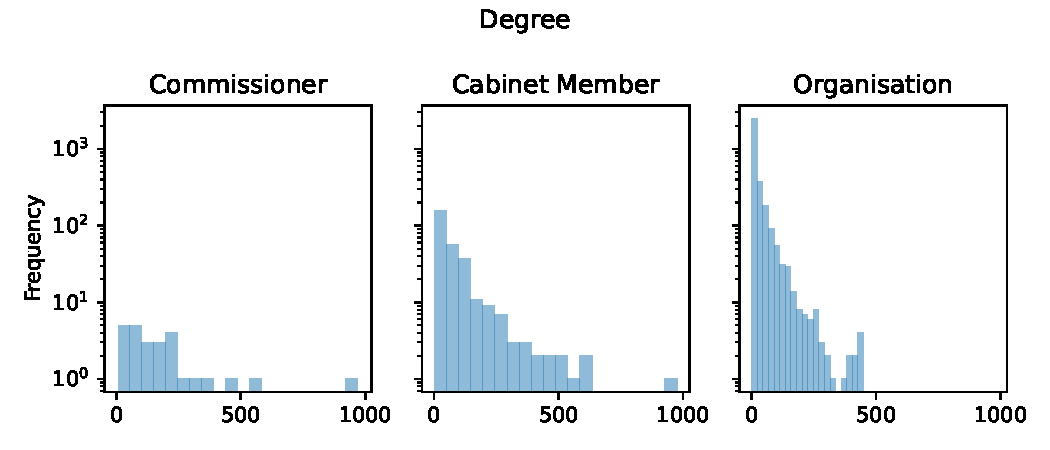
\includegraphics[scale=0.6]{../Programs/Figures/Degree.pdf}\\
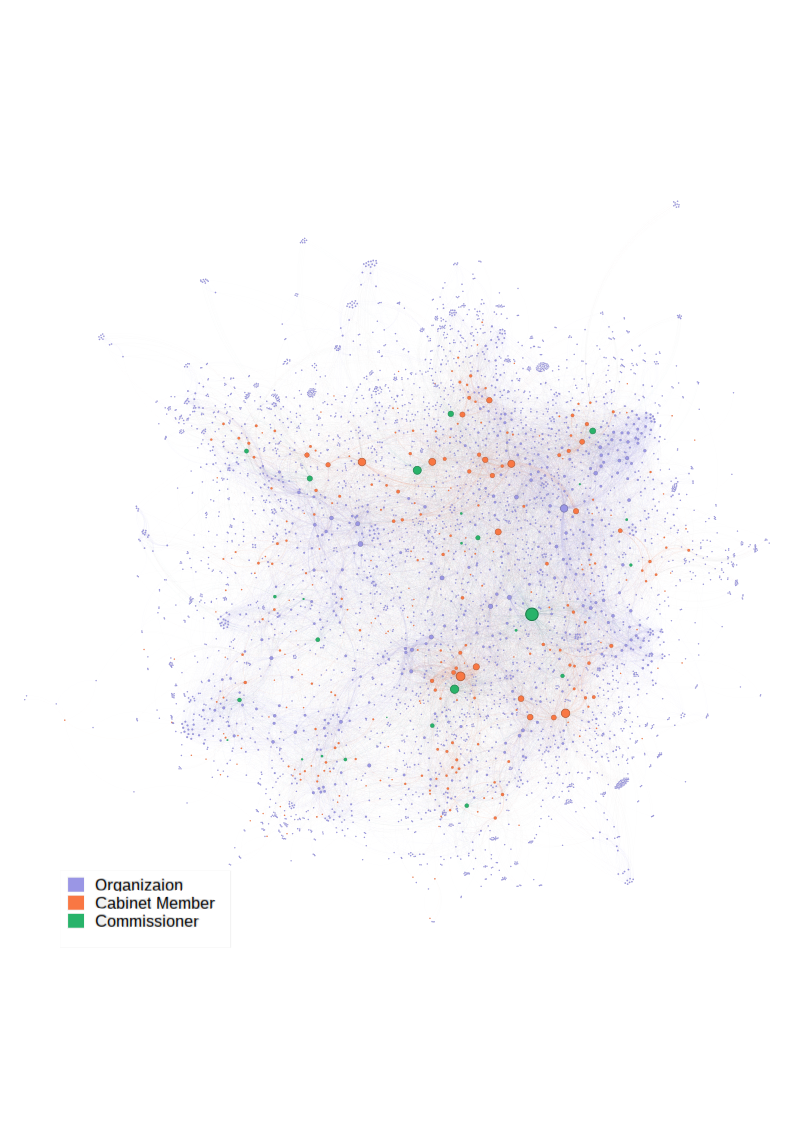
\includegraphics[scale=0.5]{../Programs/Figures/Degree.png} 

\subsection{Betweenness}
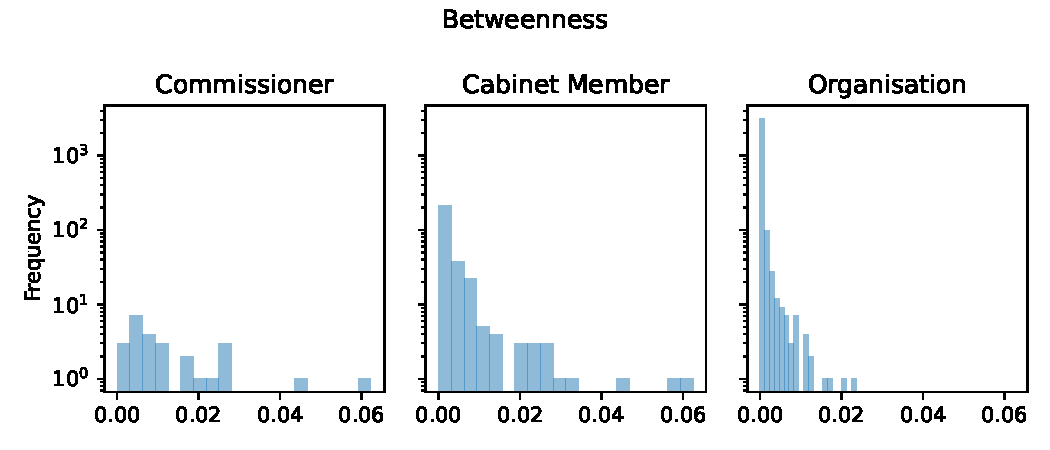
\includegraphics[scale=0.6]{../Programs/Figures/Betweenness.pdf}\\
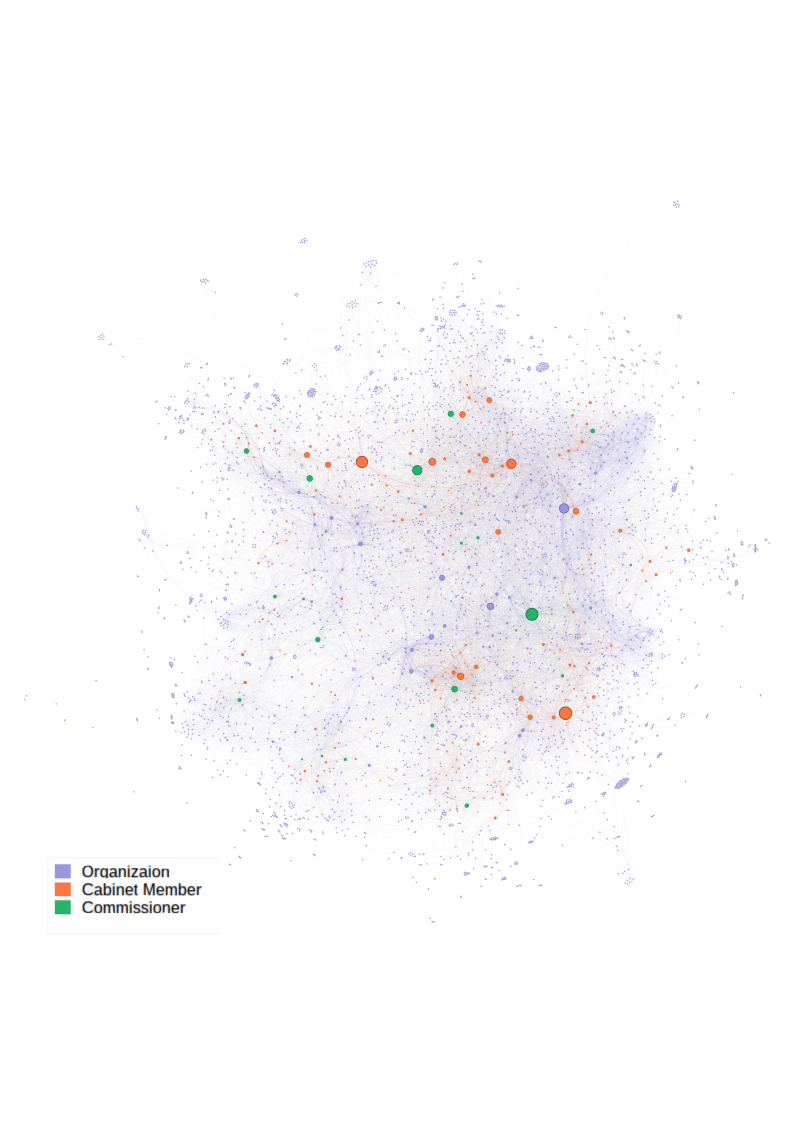
\includegraphics[scale=0.5]{../Programs/Figures/Betweenness.png} 

\subsection{Eigenvector}
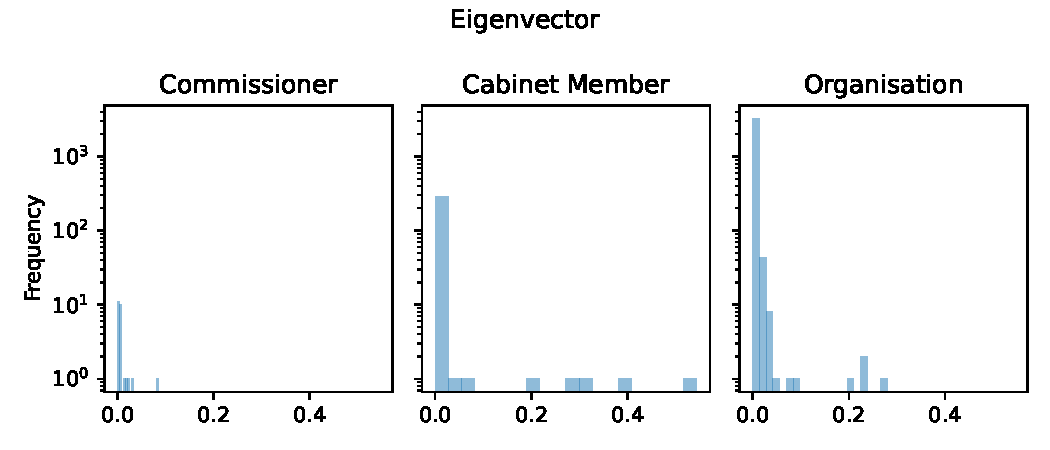
\includegraphics[scale=0.6]{../Programs/Figures/Eigenvector.pdf}\\
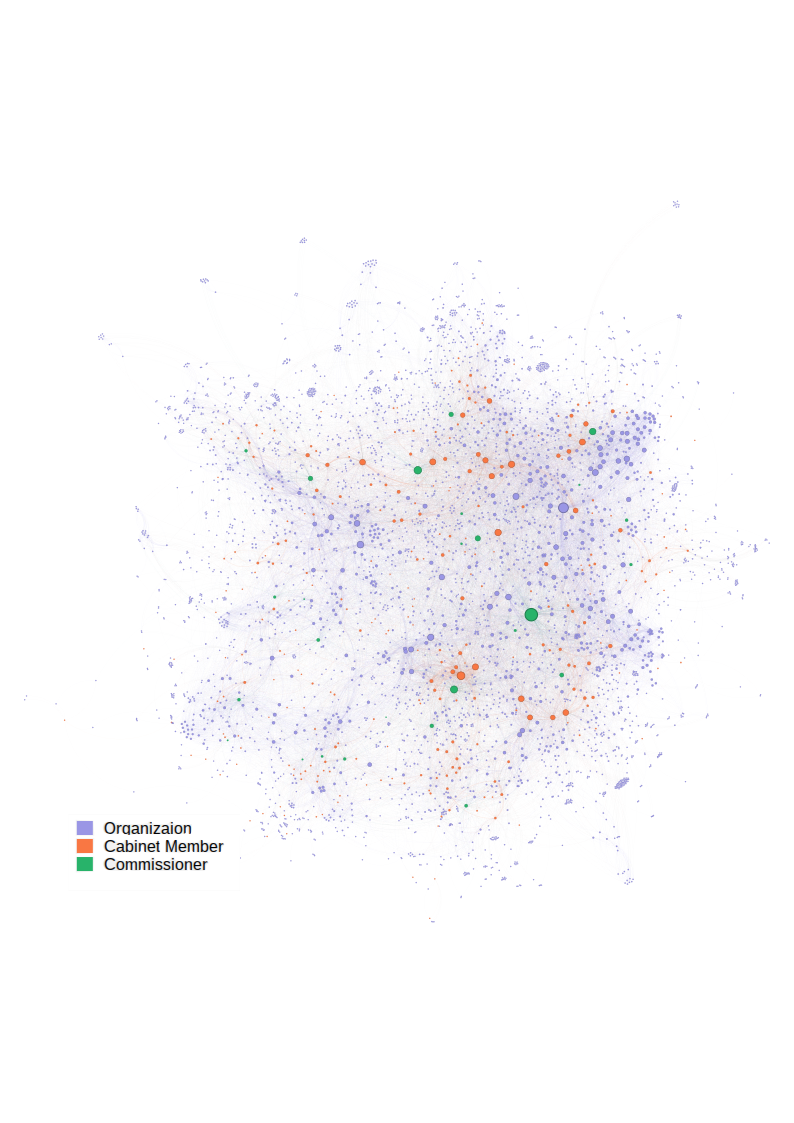
\includegraphics[scale=0.5]{../Programs/Figures/Eigenvector.png} 

\section{Correlation between E.U. grant and centralities}
restrict graph to organisation appearing the E.U. transparency register. \\
Number of nodes = 3637 \\
The network still connected \\
\begin{tabular}{|ccccc|}
\hline
             &Members FTE  &Eigenvector   & Degree  &Betweenness\\
E.U. Grants  &0.002598    &0.008545  &0.028295     &0.015429\\
\hline
\end{tabular}  \\
$\Rightarrow$ No significant correlation

\end{document}
